\newpage
\section{Power Sensor}
The purpose of this block is to measure the electrical power delivered to the car's propulsion system. The power sensor must be able to measure both the delivered voltage V and  current I, as the power P is given by:
\begin{equation}
	P = V \cdot I
\end{equation}

\subsection{Design}
The current is measured using a Hall-effect based current transducer of the type LTS 15-NP. The internal circuit of the component is seen on Figure \ref{fig:LTS_operating_principle} below. The transucer measures the strength of the magnetic field induced by the input current and converts it to a voltage. This voltage is amplified and given as the transducer's output. The internal amplifier must be supplied with 5 VDC in order for the transducer to measure properly.

\begin{figure}[H]
	\centering
	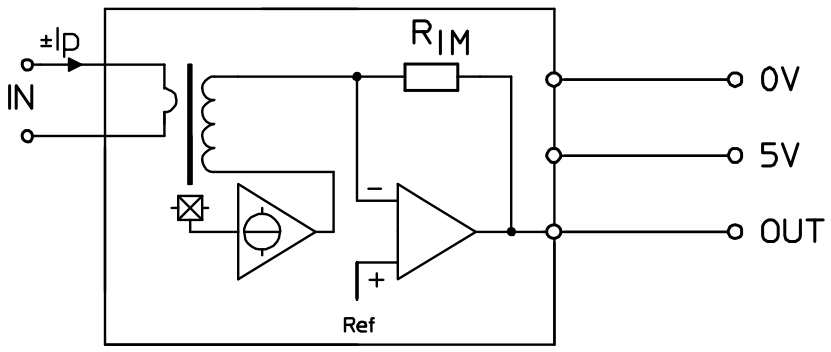
\includegraphics[width=0.5\linewidth]{Hardware/Pictures/LTS_circuit}
	\caption{LTS 15-NP Operating principle}
	\label{fig:LTS_operating_principle}
\end{figure}

This type of transducer measures the induced magnetic field around the input conductor and converts it to a voltage on the output. The strength of the field around the conductor depends on the current inside
\begin{equation}
	V_{out} = 2.5 \pm \left( 0.625 \cdot \frac{I_{P}}{I_{PN}} \right)
\end{equation}

\begin{figure}[H]
	\centering
	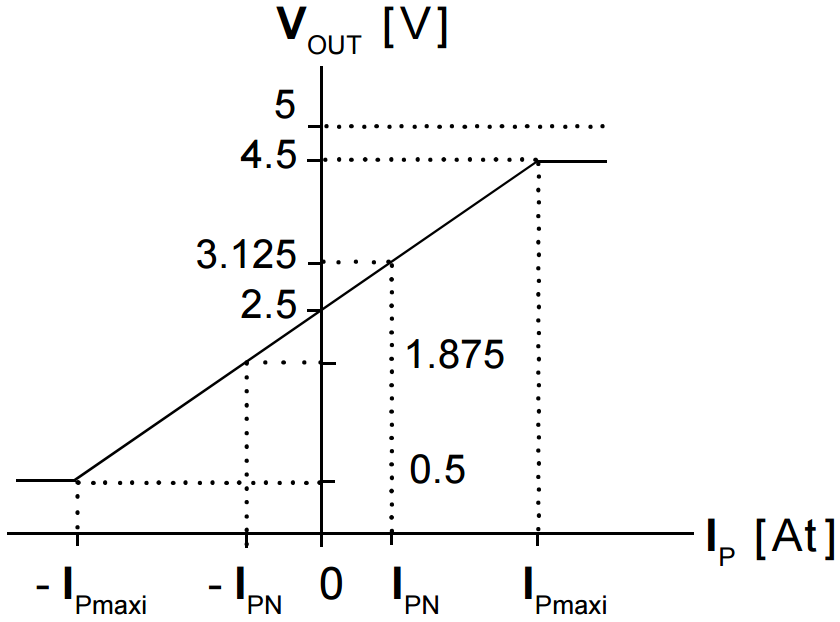
\includegraphics[width=0.5\linewidth]{Hardware/Pictures/LTS_output}
	\caption{LTS 15-NP Output voltage}
	\label{fig:LTS_output}
\end{figure}

\subsection{Implementation}
Text

\subsection{Unity test}
Text